Accurate simulations of all production processes have crucial importance to make decisions aimed to speed up the performance improvement of a shop floor. 
Applying discrete simulation techniques to a traditional shop floor can be a resource and time consuming process because of the initial data inaccuracies. 
Furthermore, even small variations of production parameters can lead to divergent simulation results compared to the actual system.

In the industry 4.0 context, the shop floor is made by self-monitoring production machines and robots, namely CPS, with the capability to share their own state information with other stakeholders. Through a connection layer, this information can be exchanged and stored and used for achieving more realistic simulation input data which, in turn, leads to more accurate forecasting capabilities. In this way, the factory behavior can be accurately predicted in advance. Moreover, thanks to this quasi real-time mirroring of real elements into their virtual representation, it is possible to simulate on current data thus exploiting simulation potentials not only in the factory design and planning phase but also in the operative one. This allows to perform what-if analysis on the current production situation in order to support decision-making processes aimed at improving performances typically outside the boundaries of simulation such as ensuing the on-time delivery of customer orders or reallocating production resources to balance the current production.

In order to allow the component to easily adapt to the possible evolution of the general architecture and of the surrounding modules, the main axes of variation for the \textit{Real-to-Digital Synchronization} problem have been identified. 
In particular, changes are expected to happen in the transmission channel and in the data format of the transmitted information.

On the other hand, it is assumed that the part responsible for the update of the simulation data model should not be subject to substantial modifications.

Figure~\ref{fig:realToDigitalComponentDia} shows the internal structure of the Real to Digital Synchronization Component that is articulated in three parts:
\begin{description}
\item[Data Client], this component is responsible for carrying the information from the physical to the digital world
\item[Format Manager] responsible of managing the data format
\item[Business Logics Manager] responsible of organizing the data in the Simulation \textit{Model Repository}
\end{description}

The following sections describe in detail each internal component.


\begin{figure}
  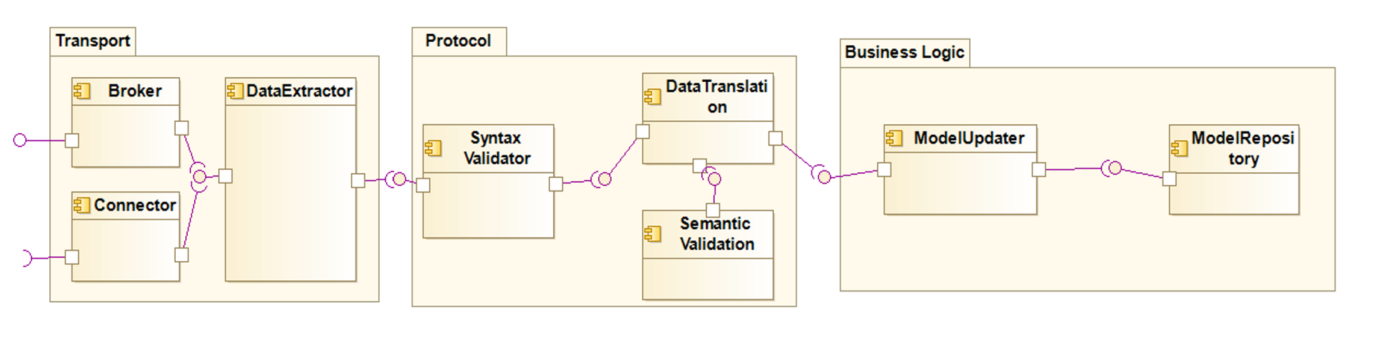
\includegraphics[width=\linewidth]{images/diagramComponent.PNG}
  \caption{Real to Digital Synchronization Component Diagram}
  \label{fig:realToDigitalComponentDia}
\end{figure}

\subsection{Data Client Component}
The main responsibility of this component is to provide a way to access the real data from the plant. This is achieved in two ways:
\begin{enumerate}
\item The first way is to access the data through a registered broker in a PUSH mode, meaning that the client is notified if new data is available. 
An example of data Broker might be MQTT or Kafka.
\item The second way is to send a request using a client named in Figure 5 as “Connector” in a PULL mode, meaning that the client is responsible for asking if new data is available. An example of Connector can be a HTTP Client.
\end{enumerate}
Both the data connection modes communicate with the \textit{Data Extractor} component, which is responsible of extracting information sent through the communication channel. 
The output of this component is a pure SenML\textbf{XXX add ref here XXS} data structure. 
The advantage of this approach is that technologies responsible for communicating the message can be decoupled from the content of the message itself. 
By replacing the particular broker or connector, indeed, the component can be adapted to any communication protocol. 
A prototype of this component is available in the Test Environment that is presented in section  5. In that version, the Data Client uses a subscription to a Kafka Channel that provides the functionalities of Broker and DataExtractor.

\subsection{Format Manager Component}
The vendor of each CPS will be responsible for defining the content of the message and the transmission format. 
For this reason, the component will have to deal with this type of issue.
This component receives from the \textit{Data Client} a message containing the incoming serialized information from the shop floor. 
This message undergoes a first syntax check using a specific JSON-schema. 
Afterwards the whole message is parsed by the \textit{Data Translator}, where a second check about the semantics is performed. 
Finally, the information is translated into an internal format required by the next component. 
Sensor ML is a specification to define sensor measurement and it provide the possibility of being represented by different formats including XML and JSON.

\subsection{Business Logics Manager Component}
The main responsibility of this component is to map the data contained in the sensor message with the specific data model instantiated in the model repository component.
After the message parsing phase, the shop floor data is validated and is available for the comparison with the corresponding model repository data. For each sensor the corresponding data should be prepared and installed in the model in advance. Vendors will be able to access the data model using an interface that can guide them in modelling the content in the digital component.

\subsection{Real-to-Digital-Synchronization Deploy}
In order to allow any vendor to create their own implementations of real to digital, a graphical interface has been developed in the project. Using a wizard, the graphical interface allows to manage the behaviour of that component. 
The wizard is organized in the following steps:
\begin{enumerate}
\item Download Prototype: In this step, the vendor responsible for the real-to-digital of its CPS can download a prototype containing the framework classes needed to implement the sub-components described in the previous sections. The package also contains JSON parsing libraries to allow vendors an easier configuration.
\item Upload: Once the component development is complete, the vendor can upload their own binary file (.jar) to the platform.
\item Pairing: through this interface the vendor has the possibility to see the CPS currently connected to the platform and also sees the real to digital drivers available. The data source (CPS) and its interpretation (real-to-digital driver) can thus be associated. It is possible to associate a different driver to each CPS or reuse an existing one according to the use case.
\item Activation: arrived at this point the CPSs connected to the platform have been associated with the real to digital drivers. As the last step is just to activate the CPS so as to allow the connection and start receiving the synchronization of data. The CPS can be deactivated at any time in order to allow, for example, updates to the synchronization drivers.
\end{enumerate}

\begin{figure}
  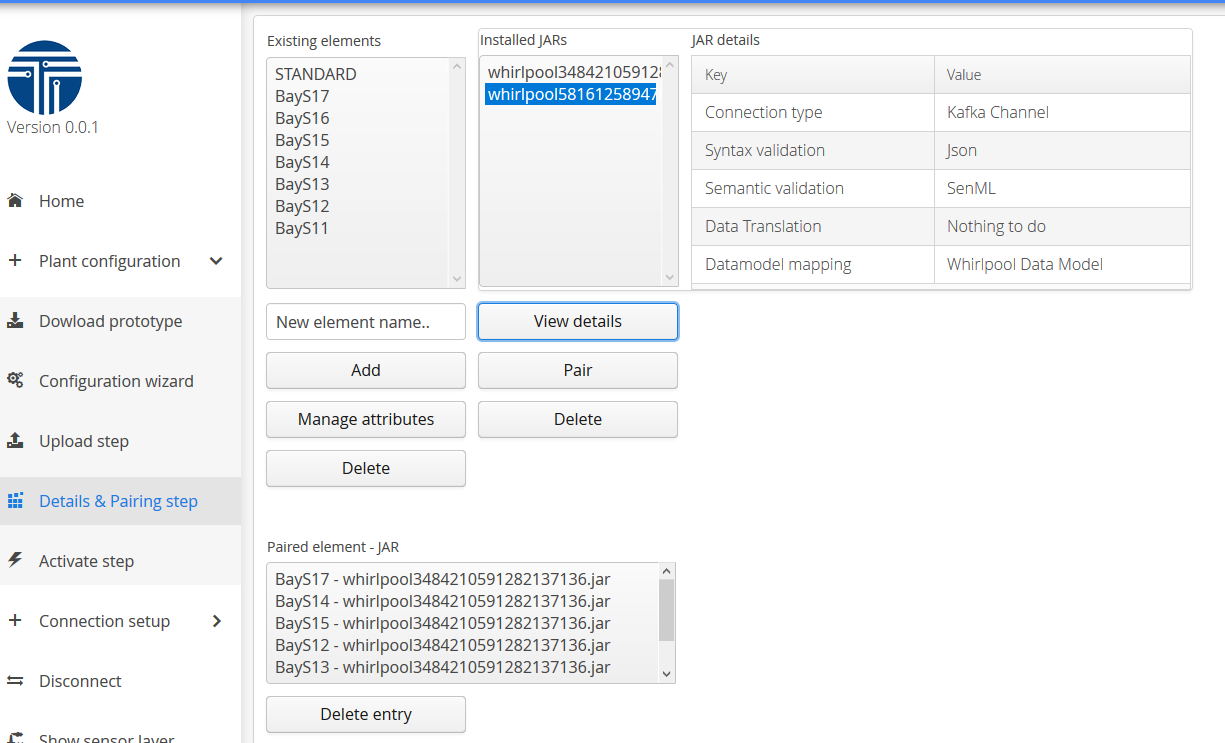
\includegraphics[width=\linewidth]{images/wizard.PNG}
  \caption{Real to Digital Synchronization wizard}
  \label{fig:wizard}
\end{figure}
